\documentclass[palace_of_the_silver_princess]{subfiles}

\begin{document}
\fontfamily{ppl}\selectfont
\clearpage

\twocolumn[{\section{Part 4: Key To The Upper Level}}]
\markright{Part 4: Key To The Upper Level}

\subsubsection{1}
\begin{quotebox}
    This watch tower room has 6 windows overlooking the surrounding
    lands. A trap door is in the center of the floor. A rope ladder lies
    to one side of it. Several arrows are embedded into the door, and a
    broken bow and a sword lay beside it.  There is a door in the east
    wall.
\end{quotebox}

After a round the players will hear scuffling and fighting noises from
the other side of the east wall door. Phrases like “Come on Briardoor, I
got her,” “no Joshua, not him” and “take that you filthy worm,” will be
heard intermixed with the other noises. If the players open the door to
investigate, bright light will fill the hallway, and all that will be
seen are three swords fighting each other as if by themselves. It is an
illusion placed there by the palace magic user to frighten intruders who
may decide to enter through the tower. The illusion will not be dis-
pelled by touch. The trap doors leads down to room \textbf{EL 38}.

\subsubsection{2}
\begin{quotebox}
    This partly intact ancient laboratory holds the remains of several
    experiments, small scraps of paper, beakers, and a variety of other
    equipment spilled across onto two large oaken tables. A beautiful
    life-size green crystal statue of a gargoyle in the northeast
    corner. A polishing cloth is draped over its shield. An empty
    bookcase is leaning against the north wall, and a destroyed bookcase
    lies on the floor near the south wall.
\end{quotebox}

The crystal gargoyle is actually a living statue and was placed here long
ago. It still serves its purpose: to defend the lab from anyone who
enters. Three scraps of paper from the pile on the tables contain spells
for a 1st level magic user (spells to be determined by the DM).

\begin{monsterbox}{Gargoyle}
    \index[monsters]{Gargoyle}
	\textit{Medium elemental, chaotic evil}\\
	\hline
	\basics[
		armorclass = {15},
		hitpoints = {52 (7d8 + 21)},
		speed = {30~ft., fly 60~ft.}]
	\hline
	\stats[
		STR = \stat{15},
		DEX = \stat{11},
		CON = \stat{16},
		INT = \stat{6},
		WIS = \stat{11},
		CHA = \stat{7}]
	\hline
	\details[
        damageresistances = {bludgeoning, piercing, and slashing from
        nonmagicalweapons that aren't adamantine},
        damageimmunities = {poison},
        conditionimmunities = {exhaustion, petrified, poisoned},
		senses = {darkvision 60~ft., passive Perception 11},
		languages = {Terran},
		challenge = {2 (450 XP)}]
	\hline
	\begin{monsteraction}[False Appearance]
		While the gargoyle remains motionless, it is indistinguishable
        from an inanimate statue.
	\end{monsteraction}
	\monstersection{Actions}
	\begin{monsteraction}[Multiattack]
		The gargoyle makes two attacks: one with its bite
        and one with its claws.
	\end{monsteraction}

    \begin{monsteraction}[Bite]
		\textit{Melee Weapon Attack:} +4 to hit, reach 5ft., one target.

        \textit{Hit:} 5 (1d6 + 2) piercing damage.
	\end{monsteraction}

    \begin{monsteraction}[Claws]
		\textit{Melee Weapon Attack:} +4 to hit, reach 5 ft., one
        target.

        \textit{Hit:} 5 (1d6 + 2) slashing damage.
	\end{monsteraction}
\end{monsterbox}

\subsubsection{3}
\begin{quotebox}
    This is a deserted room. It is now empty.
\end{quotebox}

This room once held stores of various sorts but has long since been
cleaned out.

\textbf{Monster:}
\\
\\
\\
\textbf{Treasure:}
\\
\\
\\

\subsubsection{4}
\begin{quotebox}
    A plain, single bed and a huge wooden and metal desk dominate this
    sparsely furnished bedchamber. A broom lies in one corner near a
    pile of dirt.  A tattered pair of silk bedroom slippers lie at the
    floor of the plain bed. A small chest of drawers with attached
    mirror has been turned over.
\end{quotebox}

Hiding under the bed is a small black cat. It will appear as a harmless
domesticated creature, but is actually an enchanted great cat and can
become a panther once every other hour for 10 rounds. When in small cat
form it is harmless. It will be up to the DM to keep track of the
elapsed time and determine at what times the cat will transform itself.

Sewn into the mattress of the bed are \textbf{50 gold coins} and
\textbf{3 oval shaped rubies} worth 70 gp each.

\begin{monsterbox}{Cat}
    \index[monsters]{Cat}
	\textit{Tiny beast, unaligned}\\
	\hline
	\basics[
		armorclass = {12},
		hitpoints = {2 (1d4)},
		speed = {40~ft., climb 40~ft.}]
	\hline
	\stats[
		STR = \stat{3},
		DEX = \stat{15},
		CON = \stat{10},
		INT = \stat{3},
		WIS = \stat{12},
		CHA = \stat{7}]
	\hline
	\details[
        skills = {Perception +3, Stealth +4},
		senses = {passive Perception 13},
		languages = {---},
		challenge = {0 (10 XP)}]
	\hline
	\begin{monsteraction}[Keen Smell]
        The cat has advantage on Wisdom (Perception) checks that rely on
        smell.
	\end{monsteraction}
	\monstersection{Actions}
    \begin{monsteraction}[Claws]
		\textit{Melee Weapon Attack:} +0 to hit, reach 5 ft., one
        target.

        \textit{Hit:} 1 slashing damage.
	\end{monsteraction}
\end{monsterbox}

\begin{monsterbox}{Panther}
    \index[monsters]{Panther}
	\textit{Medium beast, unaligned}\\
	\hline
	\basics[
		armorclass = {12},
		hitpoints = {13 (3d8)},
		speed = {50~ft., climb 40~ft.}]
	\hline
	\stats[
		STR = \stat{14},
		DEX = \stat{15},
		CON = \stat{10},
		INT = \stat{3},
		WIS = \stat{14},
		CHA = \stat{7}]
	\hline
	\details[
        skills = {Perception +3, Stealth +6},
		senses = {passive Perception 14},
		languages = {---},
		challenge = {1/4 (50 XP)}]
	\hline
	\begin{monsteraction}[Keen Smell]
        The panther has advantage on Wisdom (Perception) checks that rely on
        smell.
	\end{monsteraction}

    \begin{monsteraction}[Pounce]
        If the panther moves at least 20 feet straight toward a creature
        and then hits it with a claw attack on the same turn, that
        target must succeed on a DC 12 Strength saving throw or be
        knocked prone. If the target is prone, the panther can make one
        bite attack against it as a bonus action.
	\end{monsteraction}
	\monstersection{Actions}
    \begin{monsteraction}[Bite]
		\textit{Melee Weapon Attack:} +4 to hit, reach 5 ft., one
        target.

        \textit{Hit:} 5 (1d6 + 2) piercing damage.
	\end{monsteraction}

    \begin{monsteraction}[Claw]
		\textit{Melee Weapon Attack:} +4 to hit, reach 5 ft ., one
        target.

        \textit{Hit:} 4 (1d4 + 2) slashing damage.
	\end{monsteraction}
\end{monsterbox}

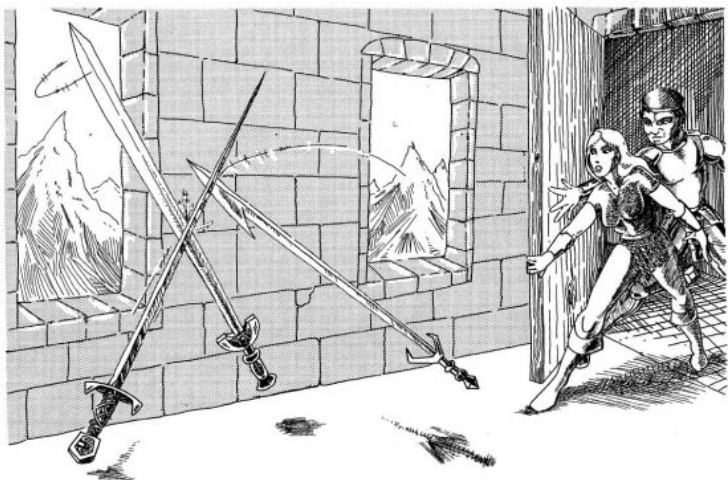
\includegraphics[width=\columnwidth]{img/trick_fight.png}

\subsubsection{5}
\begin{quotebox}
    This is a deserted room. It is empty.
\end{quotebox}

This room once held supplies and stores of various sorts but has long
since been emptied.

\textbf{Monster:}
\\
\\
\\
\textbf{Treasure:}
\\
\\
\\

\subsubsection{6}
\begin{quotebox}
    A huge, ornate, once lavishly decorated double canopy bed is
    directly across from the set of double doors. The bed posts
    resemble vines, nymphs, and birds all intertwined. The bed is
    covered in dusty, dull red velvet. Arrases line three of the walls
    with lovely and peaceful scenes of maidens riding on unicorns,
    playing in still pools that abound with plant life, and singing
    under starry skies lighted by a full moon. To either side of the
    door is a large hand carved chest of drawers, both with mirrors that
    are veined in silver. A small cushioned chair and matching footstool
    are at the end of the bed. On the footstool is a small makeup
    pallette and pestle.
\end{quotebox}

This was Lady Argenta’s room. It has remained untouched by man or
monster since the day she left it. The furniture and cloth here as well
as in the rest of the palace is rotten and of no value. All the drawers
have been emptied; and no clues or other information can be gained. The
makeup pallette is enameled in gold and was used for crushing colored
powders for eye makeup (1000 gp).

The view from the windows is into an overgrown garden.

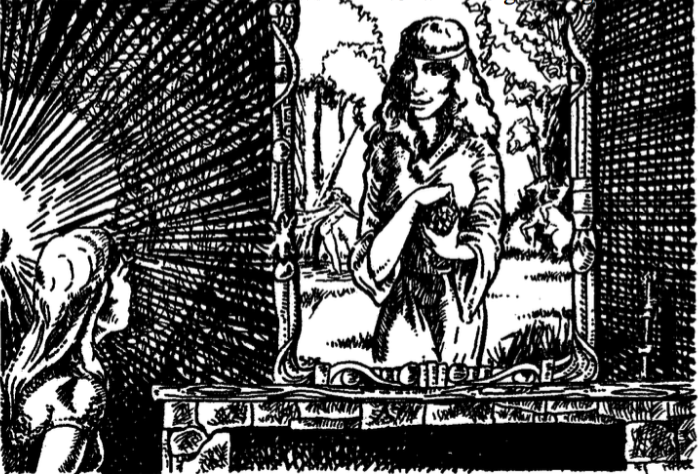
\includegraphics[width=\columnwidth]{img/lady.png}

\subsubsection{7}
\begin{quotebox}
    Several chairs and tables circle the fireplace in this room. A worn rug
    lies rolled up in one corner, and 3 knitting baskets sit beside it. On a
    small table near the fireplace is a small tea cup and saucer. Hanging
    over the fireplace is a portrait of Lady Argenta. She is holding a
    beautiful blood red ruby the size of an apple. Her smile betrays a hint
    of mischievousness.
\end{quotebox}

The only thing of value in the room is the tea cup. It is a magical
singing tea cup. When lifted off the saucer, the cup will begin to
randomly sing one of the 100 songs it knows.

\textbf{Monster:}
\\
\\
\\

\subsubsection{8}
\begin{quotebox}
    Shelves line this room. They are all empty now. A broken bedwarmer
    lays next to a small table and chair in the center of the room.
\end{quotebox}

\textbf{Monster:}
\\
\\
\\
\textbf{Treasure:}
\\
\\
\\
\textbf{Trap:}
\\
\\
\\

\subsubsection{9}
\begin{quotebox}
    This small room is lined with hangers and hooks. A chest of drawers
    is against the east wall.
\end{quotebox}

This was Lady Argenta’s closet. It is now empty of clothes or other
valuables.

\textbf{Monster:}
\\
\\
\\

\subsubsection{10}
\begin{quotebox}
    The walls of this lovely bathing room are painted with peaceful
    scenes of spring and summer. The ceiling and floor are mirrored and
    the floor retains some of its original polish. An ornate marble and
    silver enameled oval bathtub is against the eastern wall. A silver
    enameled towel rack standing next to the tub holds the remains of a
    thick towel and wash cloth. Many small and lovely soft soap
    containers are scattered randomly about the room. Bath oil pearls
    litter the now empty tub. At the head of the tub is a delicately
    sculpted tray centered with a small vase. It is decorated by three
    sets of three small gems. Each set of three is a different color —
    red, blue, and yellow.
\end{quotebox}

After one round, an ubue will enter from room \textbf{UL 11} to
investigate the noise in the bathing room. If there are more than 3
opponents, he will summon help from the remaining two ubues in room
\textbf{UL 11}. If the party is too strong, the monsters will retreat
into room \textbf{UL 11}.

The tray at the head of the tub is used to create water for bathing. The
magic works like this: Two red stones placed on the tray create hot
water, two yellow stones bring cold, and two blue ones remove it. Mix a
yellow and a red and the result is luke warm water. The blue ones only
work with each other. The tub will fill to capacity in 3 rounds. It will
empty in 1 round.

\begin{monsterbox}{Ubue}
    \index[monsters]{Ubue}
	\textit{Medium humanoid, true neutral}\\
	\hline
	\basics[
		armorclass = {10},
		hitpoints = {4 (1d8)},
		speed = {30~ft.}]
	\hline
	\stats[
		STR = \stat{10},
		DEX = \stat{10},
		CON = \stat{10},
		INT = \stat{10},
		WIS = \stat{10},
		CHA = \stat{10}]
	\hline
	\details[
		senses = {passive Perception 10},
		languages = {Common},
		challenge = {0 (10 XP)}]
	\hline
	\monstersection{Actions}
    \begin{monsteraction}[Club]
		\textit{Melee Weapon Attack:} +2 to hit, reach 5 ft., one
        target.

        \textit{Hit:} 2 (1d4) bludgeoning damage.
	\end{monsteraction}
\end{monsterbox}

\subsubsection{11}
\begin{quotebox}
    Three makeshift beds are lined against the south wall. A table with
    three chairs, and a huge stew pot sit near the fireplace. A tub
    filled with water and dishes is also near the fireplace. The walls
    are covered in portraits and other scenic paintings. Most of the
    portraits are of the Lady Argenta or of the Silver Warrior. One is
    of the red dragon, but it has been slashed in several places.
\end{quotebox}

This is the lair of three ubues. They have collected all the paintings
they could find to decorate the walls. The ubues are a family unit; one
of the ubues is female, and one is slightly smaller than the others.

The only thing of value in this room is the small chest of 40 gp hidden
under a loose brick in the fireplace.

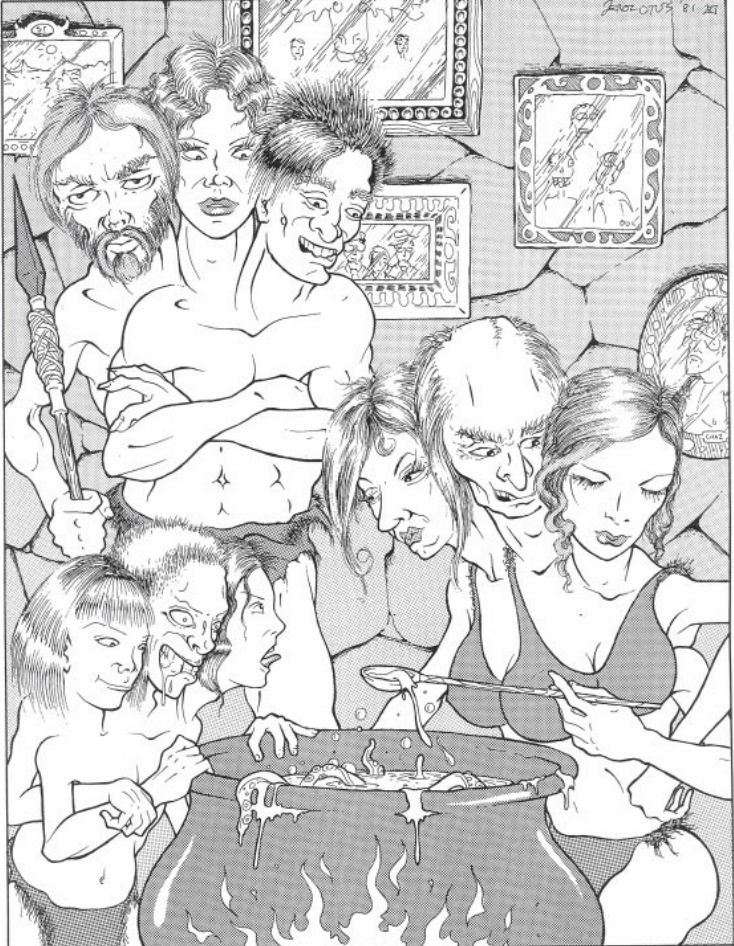
\includegraphics[width=\columnwidth]{img/ubues.png}

\subsubsection{12}
\begin{quotebox}
    This small room has only one stool and a table shoved out of the way
    against the north wall. There is a wheel on the south wall.
\end{quotebox}

This was a guard station. The wheel is used to lift the portcullis in
the hallway which is presently lowered. (A total of 20 strength points
will be needed to lift the portcullis if the wheel is not used.
Otherwise, one character with normal strength will be able to lift it.)

\textbf{Monster:}
\\
\\
\\
\textbf{Treasure:}
\\
\\
\\
\textbf{Trap:}
\\
\\
\\

\subsubsection{13}
\begin{quotebox}
    This garden is overgrown with weeds. The paths have disappeared into
    the underbrush, and the only statue is now completely grown over
    with thick purplish vines. Water can be heard, but not seen.
\end{quotebox}

Two deadly plants now inhabit this plush garden, a Jupiter blood sucker
with 6 vines, one of which is wrapped around the statue, and 8 archer
bushes. The archer bushes will attack only if disturbed. The Jupiter
blood sucker will move towards its intended victim, wrap itself around
him or her and place one of its giant leaves over the victim’s face,
thus smothering the victim while inserting its needle sharp thorns to
drain the victim’s blood.

A fountain can be found by carefully searching near the southeast
corner of the garden. The fountain has healing powers that will cure
each person once and replace all lost hit points. Any attempts to use
the water again will not be successful, nor will the healing power of
the water remain if taken out of the fountain. The water must be drunk
or lapped up straight from the fountain.

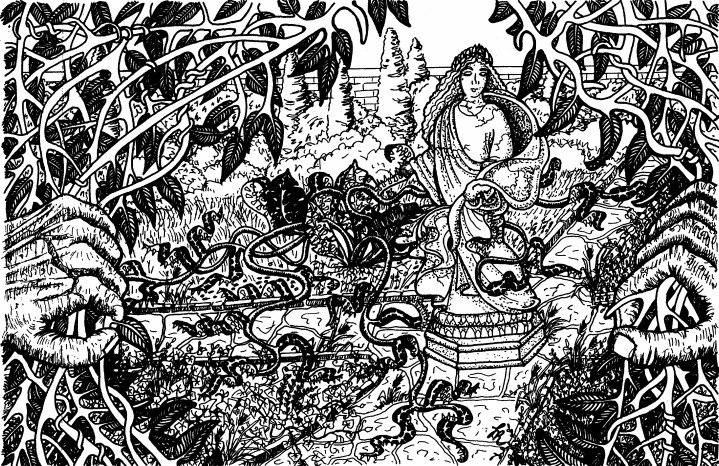
\includegraphics[width=\columnwidth]{img/garden.png}






\end{document}
